\documentclass[a0,portrait]{a0poster}

\usepackage{multicol} % This is so we can have multiple columns of text side-by-side
\columnsep=100pt % This is the amount of white space between the columns in the poster
\columnseprule=3pt % This is the thickness of the black line between the columns in the poster

\usepackage[svgnames]{xcolor} % Specify colors by their 'svgnames', for a full list of all colors available see here: http://www.latextemplates.com/svgnames-colors

\usepackage[]{algorithm2e}

\usepackage{times} % Use the times font
%\usepackage{palatino} % Uncomment to use the Palatino font

\usepackage{graphicx} % Required for including images
\graphicspath{{figures/}} % Location of the graphics files
\usepackage{booktabs} % Top and bottom rules for table
\usepackage[font=small,labelfont=bf]{caption} % Required for specifying captions to tables and figures
\usepackage{amsfonts, amsmath, amsthm, amssymb} % For math fonts, symbols and environments
\usepackage{wrapfig} % Allows wrapping text around tables and figures

\newenvironment{Figure}
  {\par\medskip\noindent\minipage{\linewidth}}
  {\endminipage\par\medskip}
	
\begin{document}

\begin{minipage}[t]{0.50\linewidth}
\vspace{-8cm}
\begin{flushleft}
\veryHuge \color{NavyBlue} \textbf{Control Allocation Problem} \color{Black}\\ % Title
\Huge\textit{AUV Thrust Allocation with Variable Constraints}\\ [1cm] % Subtitle
\end{flushleft}
\end{minipage}
%%
\hfill
%%
\begin{minipage}[t]{0.20\linewidth}
\centering

\includegraphics[width=\linewidth]{fig/logo_imtp.png}
\end{minipage}
%%
\hfill
%%
\begin{minipage}[t]{0.20\linewidth}
\centering

\includegraphics[width=\linewidth]{fig/logo_fefu.png}
\end{minipage}

\vspace{1.5cm}

\begin{minipage}[t]{0.48\linewidth}
\huge \textbf{Anton Tolstonogov}\\ % Author(s)
\huge Institute of Marine Technology Problems\\ % University/organization
\huge Far Eastern Federal University\\
\end{minipage}
%%
\hfill
%%
\begin{minipage}[t]{0.48\linewidth}
\vspace{-1.0cm}
\begin{flushleft}
\color{DarkSlateGray}\Large \textbf{Contact Information:}\\
Institute of Marine Technology Problems\\ % Address
Vladivostok, Sukhanova st. 5a\\
%Phone: +7 (950) 282 51-56\\ % Phone number
Email: \texttt{tolstonogov.anton@gmail.com}\\ % Email address
\end{flushleft}
\end{minipage}

\begin{minipage}[t]{0.48\linewidth}
\textbf{\textit{Abstract} -- Modern multipurpose autonomous underwater vehicles (AUVs) represent the next generation of robotic complexes with new technological tasks faced by scientific researchers. One method for functionality extension is installing of tunnel thrusters in addition to stern propulsion system. Thereby a vehicle obtains capability to undertaking both survey-style missions and low speed interaction with the environment. But efficiency of tunnel thruster depends strongly on vehicle velocity by a hydrodynamic aspect. The common solution of this problem is different control models and thrust allocation methods for both mission types. The unified approach of thrust allocation method is presented in this study. The method is based on solution of allocation problem by quadratic programming with variable constraints.
\newline
\textit{Keywords -- AUV, propulsion system, thruster hydrodynamic, control allocation problem, quadratic programming, interior point method}}

\color{SaddleBrown}

\begin{multicols}{2}
[
\section*{Introduction}
]
The design of control algorithm for underwater vehicles is often divided into several levels \cite{survey}. First, a high level motion control algorithm is designed to compute a vector of virtual inputs to the vehicle. Second, a control allocation algorithm is designed in order to map the vector of virtual input forces and moments into individual thruster forces $\boldsymbol{t}$ such that the total forces generated by all thrusters amounts to the commanded virtual input. Third, there is a separate low-level controller of it's thrusters in order to archive desired force.

This modularity allows the high-level motion control algorithm to be designed without detailed knowledge about the vehicle propulsion system. In addition to coordinating the effect of different thrusters in the system, issues such as thruster/fault tolerance, redundancy and control constraints are typically handed within the control allocation module. In case of over-actuated propulsion system when number of thrusters more than number of DOF controlled by vehicle, the control allocation module solves optimization problem to archive minimal power consumption of propulsion system \cite{load_balancing}.
\end{multicols}

\begin{multicols}{2}
[
\section*{Propulsion System Setup}
]
The model of the AUV ``MT-2012'' \cite{auv_mt} propulsion system was used for algorithm simulation.
The propulsion system consists of five thrusters: four thrusters located at vehicle stern with $\alpha$ angle to longitudinal axis and the vertical tunnel thruster at forward part of the vehicle (fig. \ref{fig:auv}).

The propulsion system of vehicle can be described by thrust configuration matrix $B$ \cite{book_fossen}:
\begin{equation*}
B = [\boldsymbol{b}_b, \boldsymbol{b}_l, \boldsymbol{b}_u, \boldsymbol{b}_r, \boldsymbol{b}_f]
\end{equation*}

where is $\boldsymbol{b}_d, \boldsymbol{b}_l, \boldsymbol{b}_u, \boldsymbol{b}_r$ - column vectors of stern (\textbf{d}own, \textbf{l}eft, \textbf{u}p, \textbf{r}ight) 
thrusters and $\boldsymbol{b}_f$,  - column vector of \textbf{f}orward tunnel thruster.
The column vectors in 3DOF (\textit{surge, pitch and yaw}) take the following form.
For up and down stern thrusters:
\begin{equation*}
\begin{array}{ccccc}
\boldsymbol{b}_u &= \left(\right.
c_{\alpha},&
l_z^u c_{\alpha} - l_x^u s_{\alpha},&
0
\left.\right)^T \\
\boldsymbol{b}_d &= \left(\right.
c_{\alpha},&
l_z^d c_{\alpha} - l_x^d s_{\alpha},&
0
\left.\right)^T \\
\end{array}
\end{equation*}

for left and right stern thrusters:
\begin{equation*}
\begin{array}{ccccc}
\boldsymbol{b}_l &= \left(\right.
c_{\alpha},&
0,&
l_y^l c_{\alpha} - l_x^l s_{\alpha}
\left.\right)^T \\
\boldsymbol{b}_r &= \left(\right.
c_{\alpha},&
0,&
l_y^r c_{\alpha} - l_x^r s_{\alpha}
\left.\right)^T \\
\end{array}
\end{equation*}

for the forward tunnel thruster:
\begin{equation*}
\begin{array}{ccccc}
\boldsymbol{b}_f &= \left(\right.
c_{\alpha},&
-l_x^a,&
0&
\left.\right)^T \\
\end{array}
\end{equation*}

Here $c_{\alpha}, s_{\alpha}$ are $\cos{\alpha}$ and $\sin{\alpha}$ respectively and $\boldsymbol{r}^i = [l_x^i, l_y^i, l_z^i]$ is the moment arm of $i$ thruster (where $i = u,d,l,r,f$ ). For current propulsion system due to symmetrical reasons $l_z^u = l_y^r = -l_z^d = -l_y^l = L_{zy}^{stern}$ and $l_x^u=l_x^d=l_x^l=l_x^r = L_{x}^{stern}$.

Parameters of the propulsion system is shown in table \ref{table:propulsion}.

\begin{center}
\begin{tabular}{l l l l l}
\toprule
$L_{x}^{stern}$,  $m$ & 1.88  & $\alpha$,           $grad$ & 22.5 \\
$L_{zy}^{stern}$, $m$ & 0.23  & $f_{lim}^{stern}$,  $H$    & 120.1/-68.2 \\
$l_x^{tunnel}$,   $m$ & 1.20  & $f_{lim}^{tunnel}$, $H$    & 122.1/-122.0\\
\bottomrule
\end{tabular}
\captionof{table}{\color{Green} The AUV ``MT-2012'' propulsion system parameters}
\label{table:propulsion}
\end{center}\vspace{1cm}
\end{multicols}

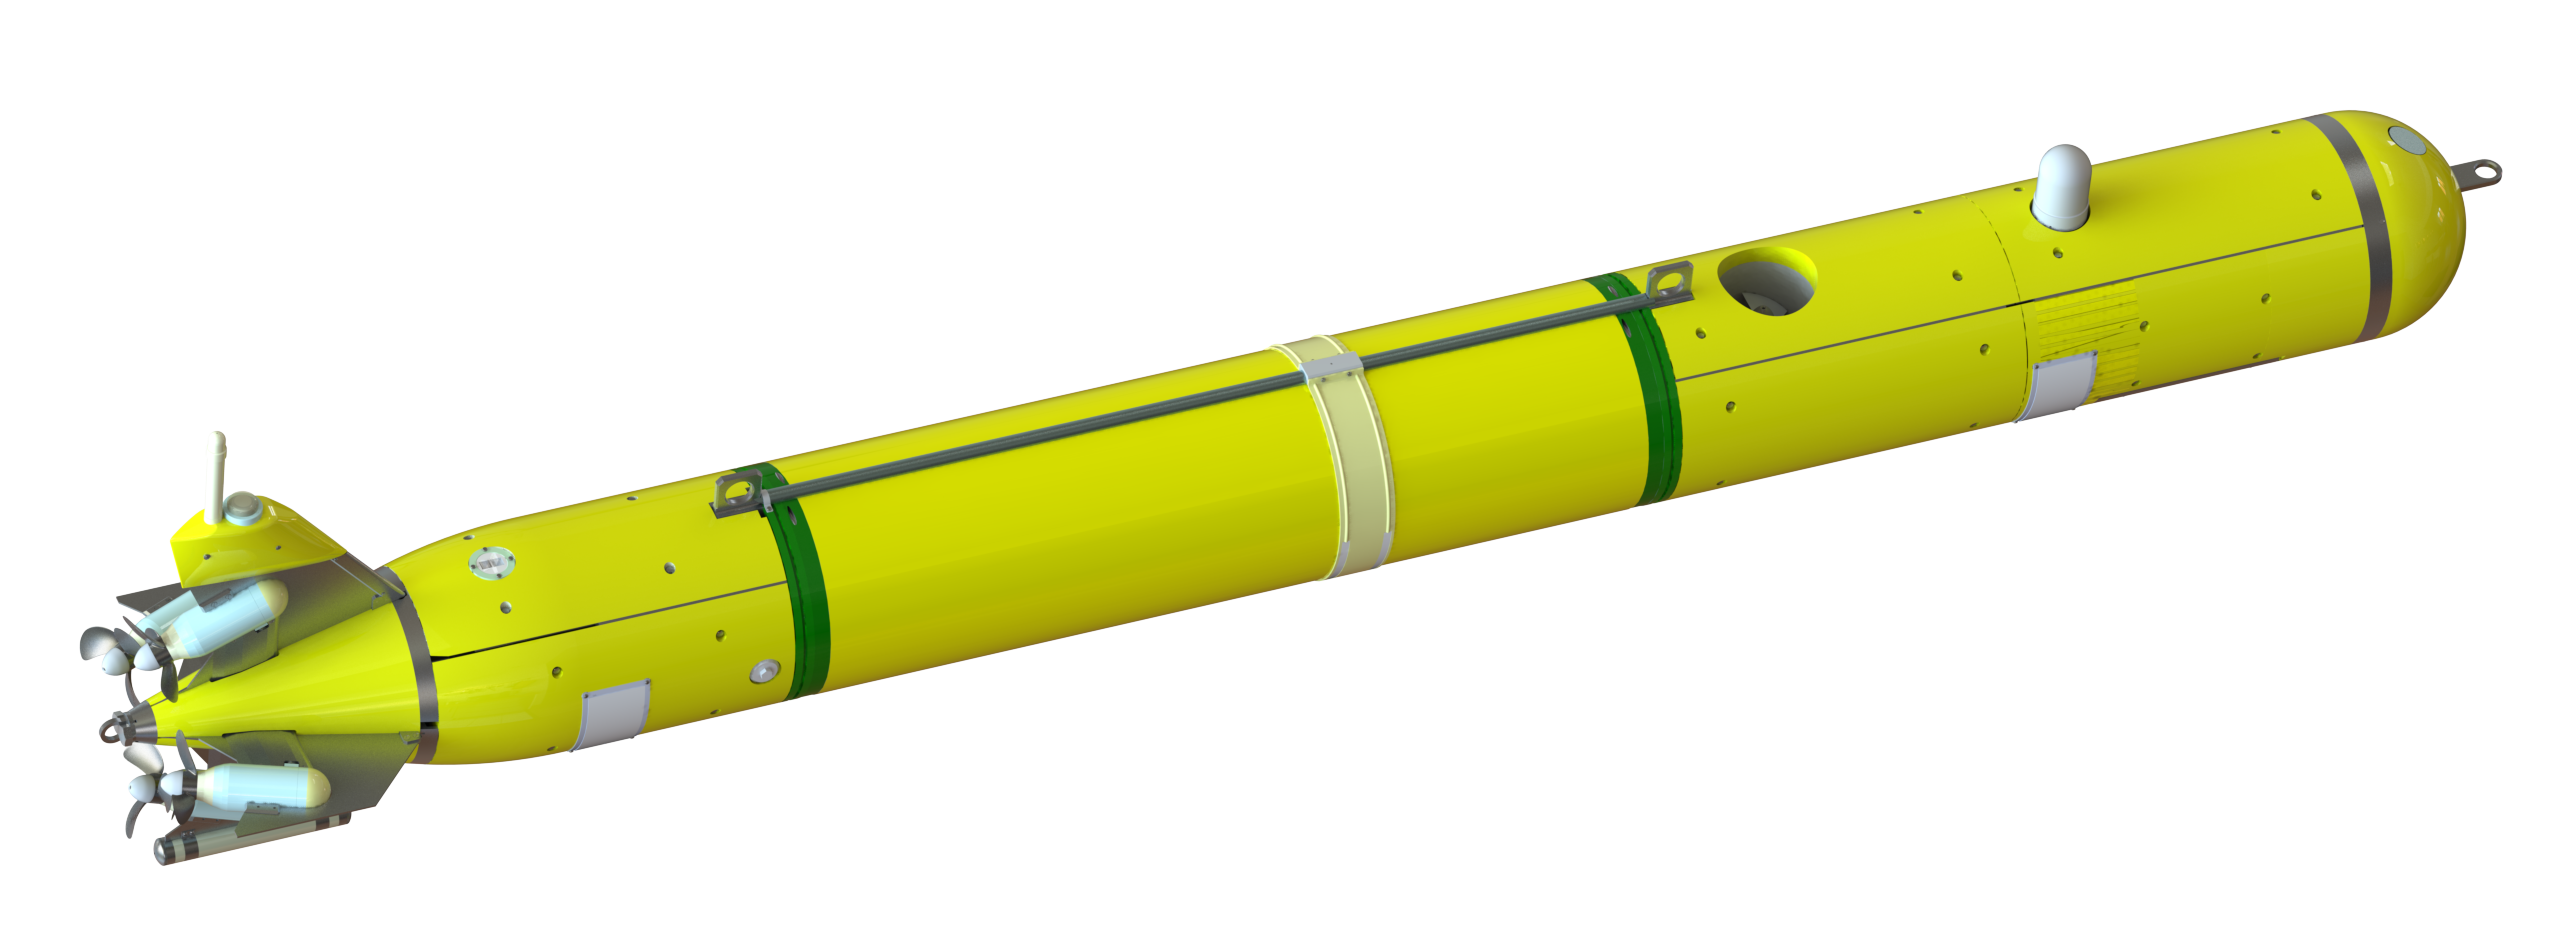
\includegraphics[width=1.0\linewidth]{fig/auv.png}
\captionof{figure}{\color{Green} Propulsion system of ``MT-2012''}
\label{fig:auv}

\begin{multicols}{2}
[
\section*{Simulation Setup}
]
The suggested algorithm of control allocation with variable constraints was tested on depth maneuvering on velocities range $[0.3...1.8]ms^{-1}$ (corresponding forward force $[3.6...129.6]H$) and pitch moment $50Hm$.

The optimal thrust allocation problem on current velocity was solved by Optimization Toolbox MATLAB. Due to $Q>0$ and $R>0$ (equation \ref{eq:problem}) this defines a convex quadratic problem in $\boldsymbol{t}$ variable and interior point method for convex optimization problem can be used.

The result of thruster allocation for different vehicle velocities is shown on fig \ref{plot}.

There is C++ implementation of convex optimization solver for embeded system. For example, light-weight library under MIT licence \cite{repo} or \cite{qp_1}.
\end{multicols}
\end{minipage}
%%
\hfill
%%
\color{SaddleBrown}
\begin{minipage}[t]{0.48\linewidth}
\begin{multicols}{2}
[
\section*{Problem Formulation}
]
Let the commanded forces and moments computed by high level motion control or vehicle operator be denoted as general vector $\boldsymbol{f} = (f_x, f_y, f_z, m_x, m_y, m_z)^T$, there are $f_i$ - force projections of i-axis and $m_i$ - moment projections of i-axis in the body-fixed coordinate frame. The NED  coordinate frame \cite{ned} is used in this work. The $x$-axis is directed along longitudinal vehicle axis from vehicle stern to forward, $y$-axis is directed along latitudinal vehicle axis from left side to right, and $z$-axis completes one to right-handed coordinate system. Assume the system is equipped with $n$ thrusters with control inputs $t_i (i = 1...n)$. This leads to a relationship between the controls $\boldsymbol{t}=(t_1,t_2,...,t_n)$ and the generalized force $\boldsymbol{f}$:
\begin{equation}
	B\boldsymbol{u} = \boldsymbol{f}
\end{equation}
where $B$ is thrust configuration matrix, it is contains location and orientation of all thrusters.

According to \cite{allocation_1}, the optimization problem with variable constraints $\boldsymbol{t}_{min}(v)$ and $\boldsymbol{t}_{max}(v)$ can be written as:

\begin{gather}
	\min\limits_{t,s} \frac{1}{2}(\boldsymbol{t}^TQ\boldsymbol{t}+\boldsymbol{s}^TR\boldsymbol{s}) \notag \\
	B\boldsymbol{t} = \boldsymbol{f} + \boldsymbol{s}\\
	\boldsymbol{t}_{min}(v) \leq \boldsymbol{t} \leq \boldsymbol{t}_{max}(v) \notag
	\label{eq:problem}
\end{gather}

Here $\boldsymbol{s}$ is a vector of slack variables used to penalize $\left|B\boldsymbol{t} - \boldsymbol{f}\right|$, $Q$, $R$ - the weight diagonal matrix for thruster and DOF prioritize respectively and $v$ - is current vehicle velocity.
\end{multicols}

\begin{multicols}{2}
[
\section*{The Model of Thruster Constraints}
]
Thrust and moment generated by a thruster can be described by formulas:
\begin{gather}
	t = K_t({\lambda})\rho n^2 D^4\notag \\
	m = K_m({\lambda})\rho n^2 D^5\notag
\end{gather}
Here $\rho$ is water density, $n$ - rotation speed of thruster propeller and $D$ is diameter of propeller. $K_t({\lambda}), K_m({\lambda})$ ($\lambda$ is advance ratio) are coefficients determined by propeller form. The functions $K_t({\lambda}), K_m({\lambda}$ can be fitted as linear function of velocity. Then stern thruster constrains can be written as:

\begin{equation}
	t_{lim}(v) = t_{lim}(0) - kv
	\label{eq:constraints_1}
\end{equation}
%Here $t_{lim}(v)$ is stern thruster constraints on velocity $v$, $k$ is coefficient determined by propeller form.

The steady state performance of the tunnel thruster can be fitted as exponential function of velocity ratio $v/v_{jet}$ \cite{thruster_tunnel}:
\begin{equation*}
	t(v) = t(0)\exp^{-c(v/v_{jet})^2}
\end{equation*}
Here $t(v)$ is the resulting force of tunnel thruster at vehicle velocity equal to $v$, $t(0)$ - thruster performance at zero vehicle velocity, $v_{jet}$ - velocity of  water jet generated by thruster.

Therefore the tunnel thruster constraints are:
\begin{equation}
	t(v)_{lim} = t(0)_{lim}\exp^{-c(\frac{v}{v_{jet,lim}})^2}
\label{eq:constraints}
\end{equation}

Where $t(v)_{lim}$ is thruster constraints during the vehicle motion at $v$ velocity and $t(0)_{lim}$ is the thruster constraints provided by bollard pull tests of the thruster.
\end{multicols}

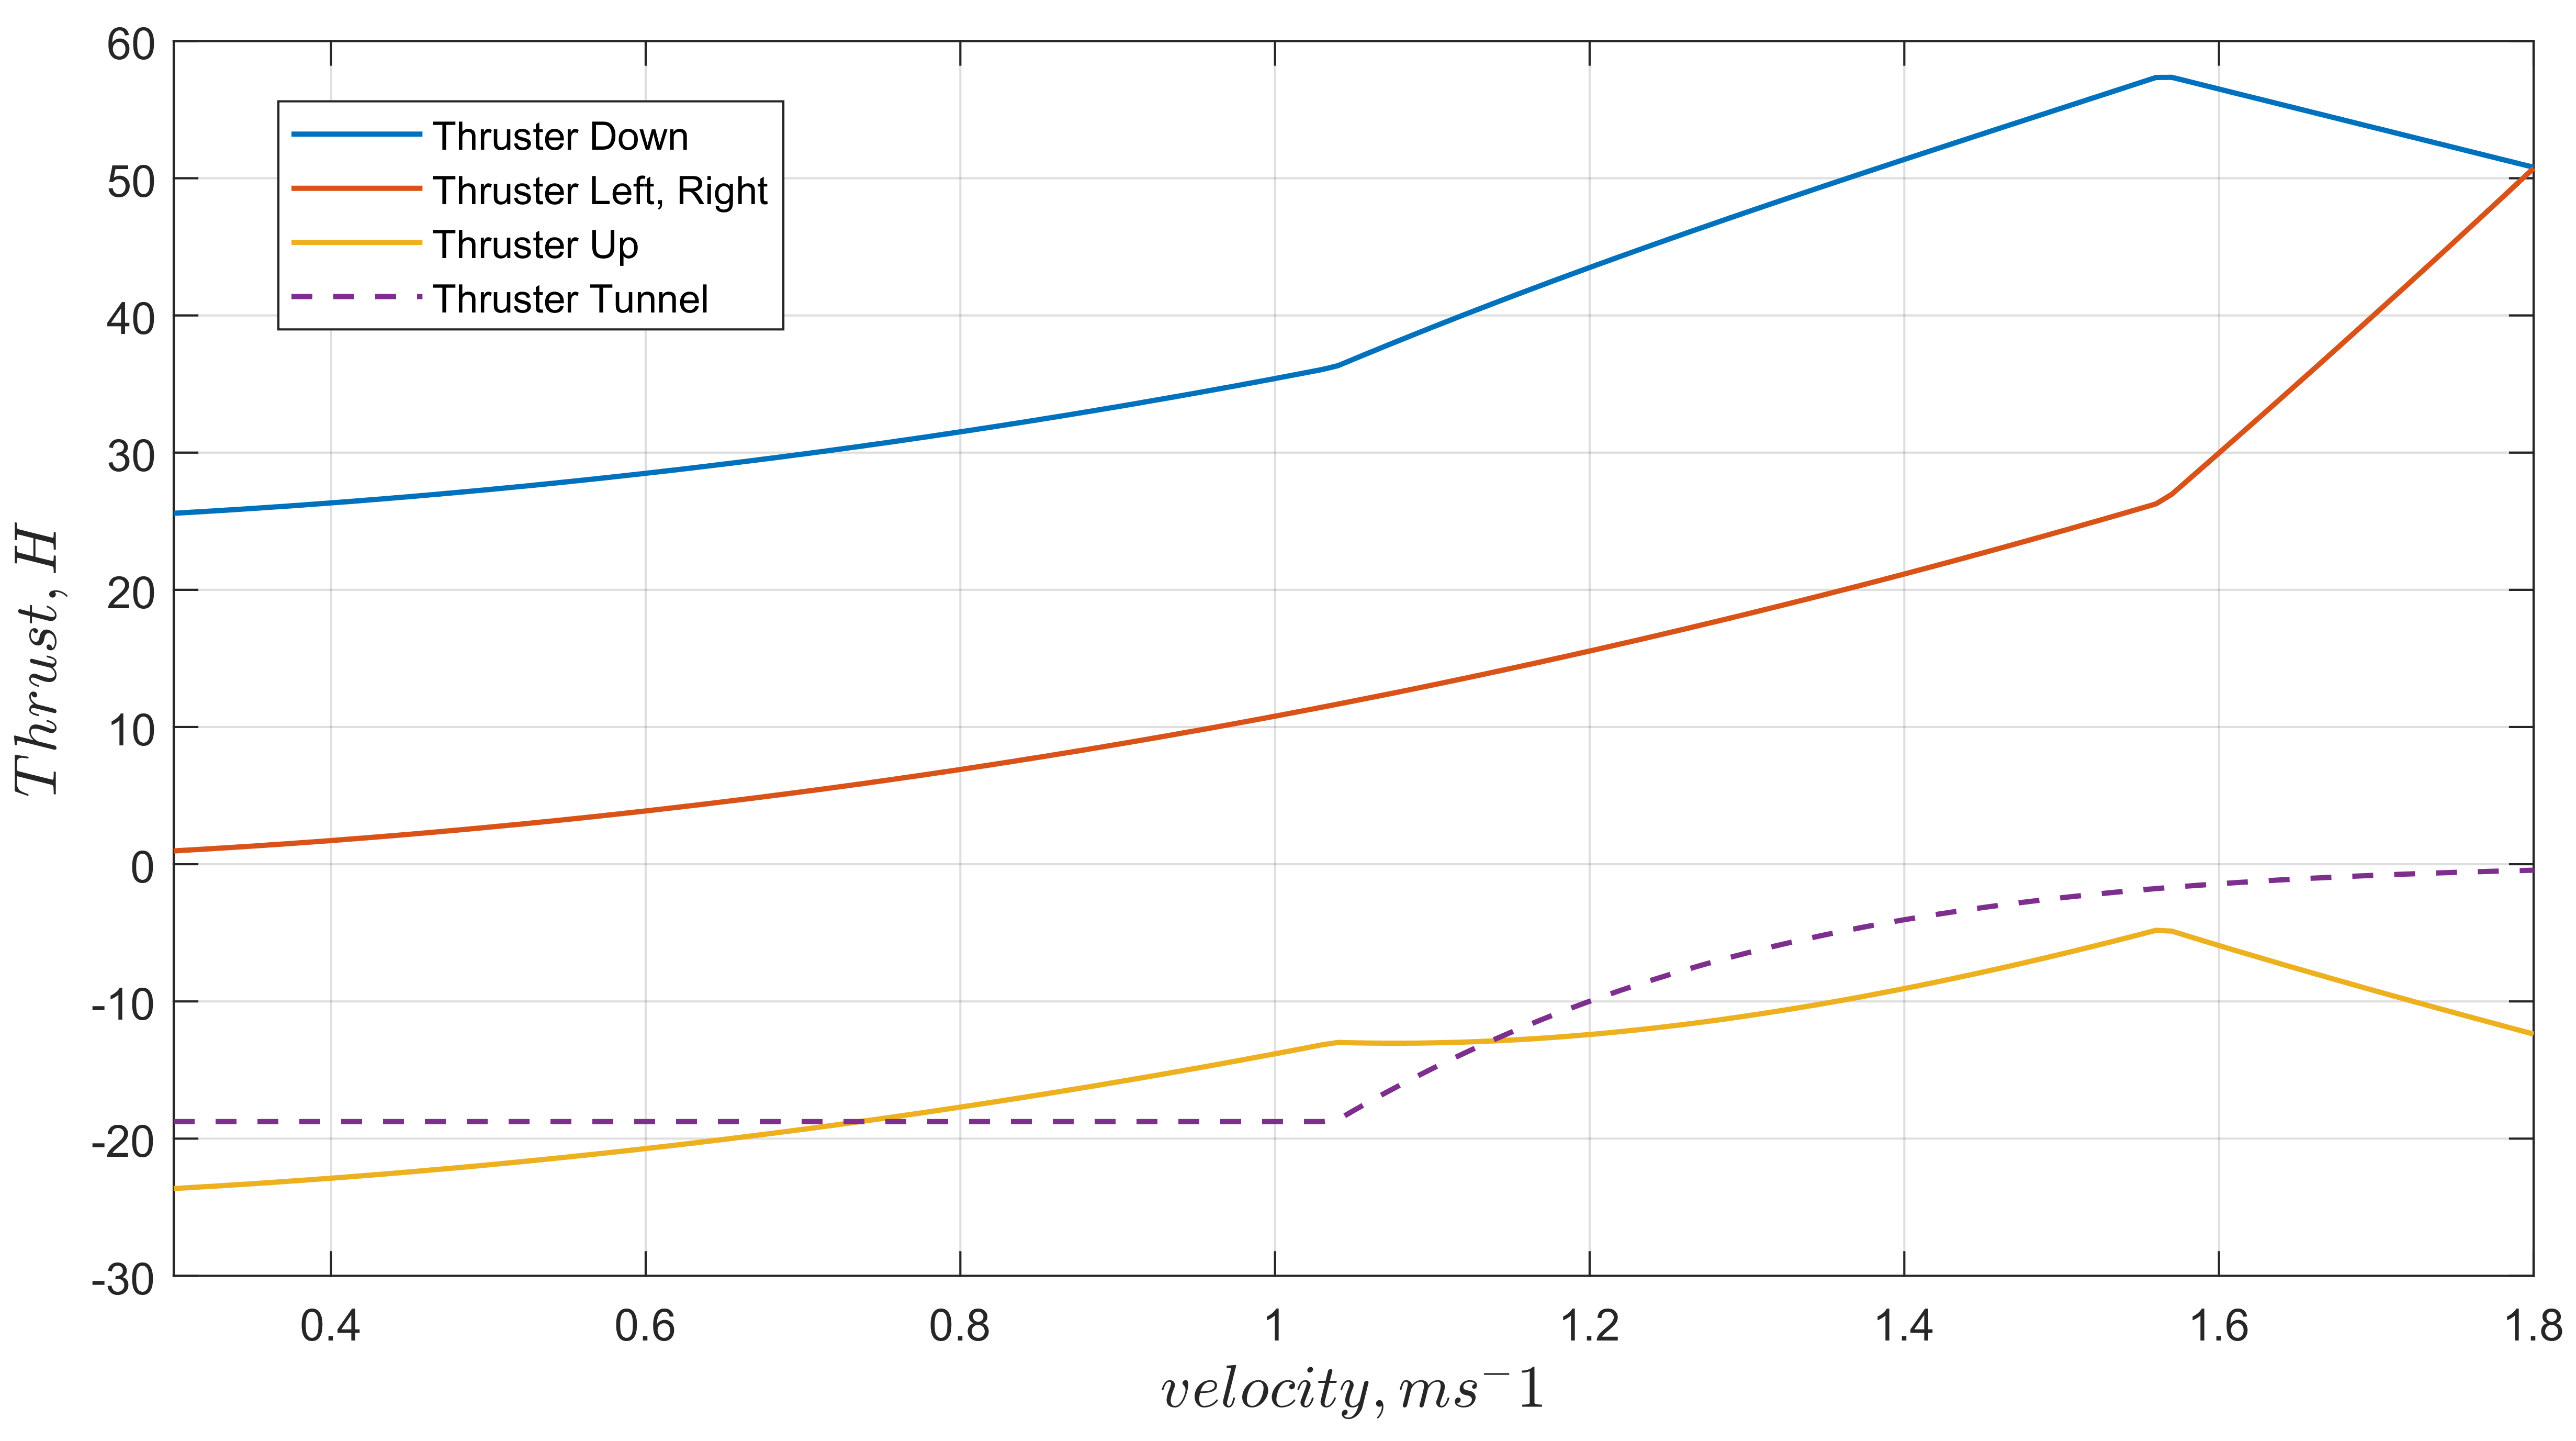
\includegraphics[width=\linewidth]{fig/Allocation_50My.png}
\captionof{figure}{\color{Green} Thrust allocation for different velocities}
\label{plot}

\section*{Conclusions}
\begin{multicols}{2}
To create multi-purpose AUV capable of undertaking both survey-stile missions and low speed interaction requires the sophisticated thruster allocation algorithms. The quadratic cost optimal approach to constrained control allocation with variable constraints is suggested. The method takes into account thrust dropping on tunnel thruster on high velocities and reallocation thrust on stern thrusters according to it. The proposed algorithm was tested on simulation model of real AUV ``MT-2012'' propulsion system.
\end{multicols}

%\color{Black}
\scriptsize
\section*{References}
\begin{multicols}{2}
\renewcommand\refname{\vskip -1cm}
\bibliographystyle{apalike} % Plain referencing style
\bibliography{bib} % Use the example bibliography file sample.bib
\end{multicols}
\end{minipage}

\end{document}